\section{Pre-Studies}
\label{chap:pre_studies}

Based on the work of Dokmanic et al. \cite{dokmanic_roomrecslam_2016} the question is now whether the RIR will be suitable for SLAM when the speaker is mounted on the robot. In the case of Dokmanic et al. \cite{dokmanic_roomrecslam_2016} described in Section \ref{sec:acoustic_slam}, the RIR is a continuous function that won't change until the speaker moves or the room will change. In this project, the speaker will move along with the robot. So the RIR as a 2D function over the room will change every time. In the pre-studies, it will be investigated if the RIR is suitable for SLAM when the speaker and microphone is at the same position.

The principle of sending a signal in a room and recording it with a microphone could be treated as an electrical system where the sent signal is the input and the recorded signal the output of the electrical system. In the concept of electrical systems, the output $y(t)$ depends on the input $x(t)$ and a function $g(t)$ which is convolved with the input in time domain. So it follows
$$
y(t) = (g * x)(t) \text{.}
$$

If the system, in our case the room, is stimulated with a Dirac impulse as input $x(t)$, $g(t)$ is the impulse response. The impulse response is hard to calculate in time domain because of the convolution $(g * t)(x)$. It's easier to calculate $G(\omega)$ in frequency space. The transformation from time domain to frequency space and back could be done with Fourier transformation. $G(\omega)$ can be calculated like
$$
Y(\omega) = G(\omega) X(\omega) \Rightarrow G(\omega) = \frac{Y(\omega)}{X(\omega)}\text{.}
$$

Obviously, the input signal can't be infinitely small. Also, because of the time-frequency uncertainty relation, an impulse has to have a certain length if a wide frequency band wants to be stimulated. For the pre-studies, we decided to use a chirp signal which is a sinusoidal function with a rise in frequency. Before calculating the impulse response, we decided to window the output with a Tukey window. The windows are overlapping slightly so that the area under the overlap is one. Each window is then Fourier transformed and the mean in frequency space is calculated. Figure \ref{fig:signal_response_example} shows an example of a chirp signal, the recorded equivalent and the impulse response in frequency space.

When looking at different phase plots of the RIR at the same position, it can be seen that the phase changes randomly. Because with the platform that is used to play the sound back, it is not possible to guarantee that the recording and sound playing starting at the same time. So there is always a random shift in time which depends on the CPU. If later needed, it may possible to compensate this shift by using cross-correlation to find the starting point of the chirp signal. But the error has to be significantly lower than 250 \si\micro s when using frequencies up to 4000 Hz which could be difficult because of the noisy recordings.

\begin{figure}[h!]
	\centering	
	\subfloat{{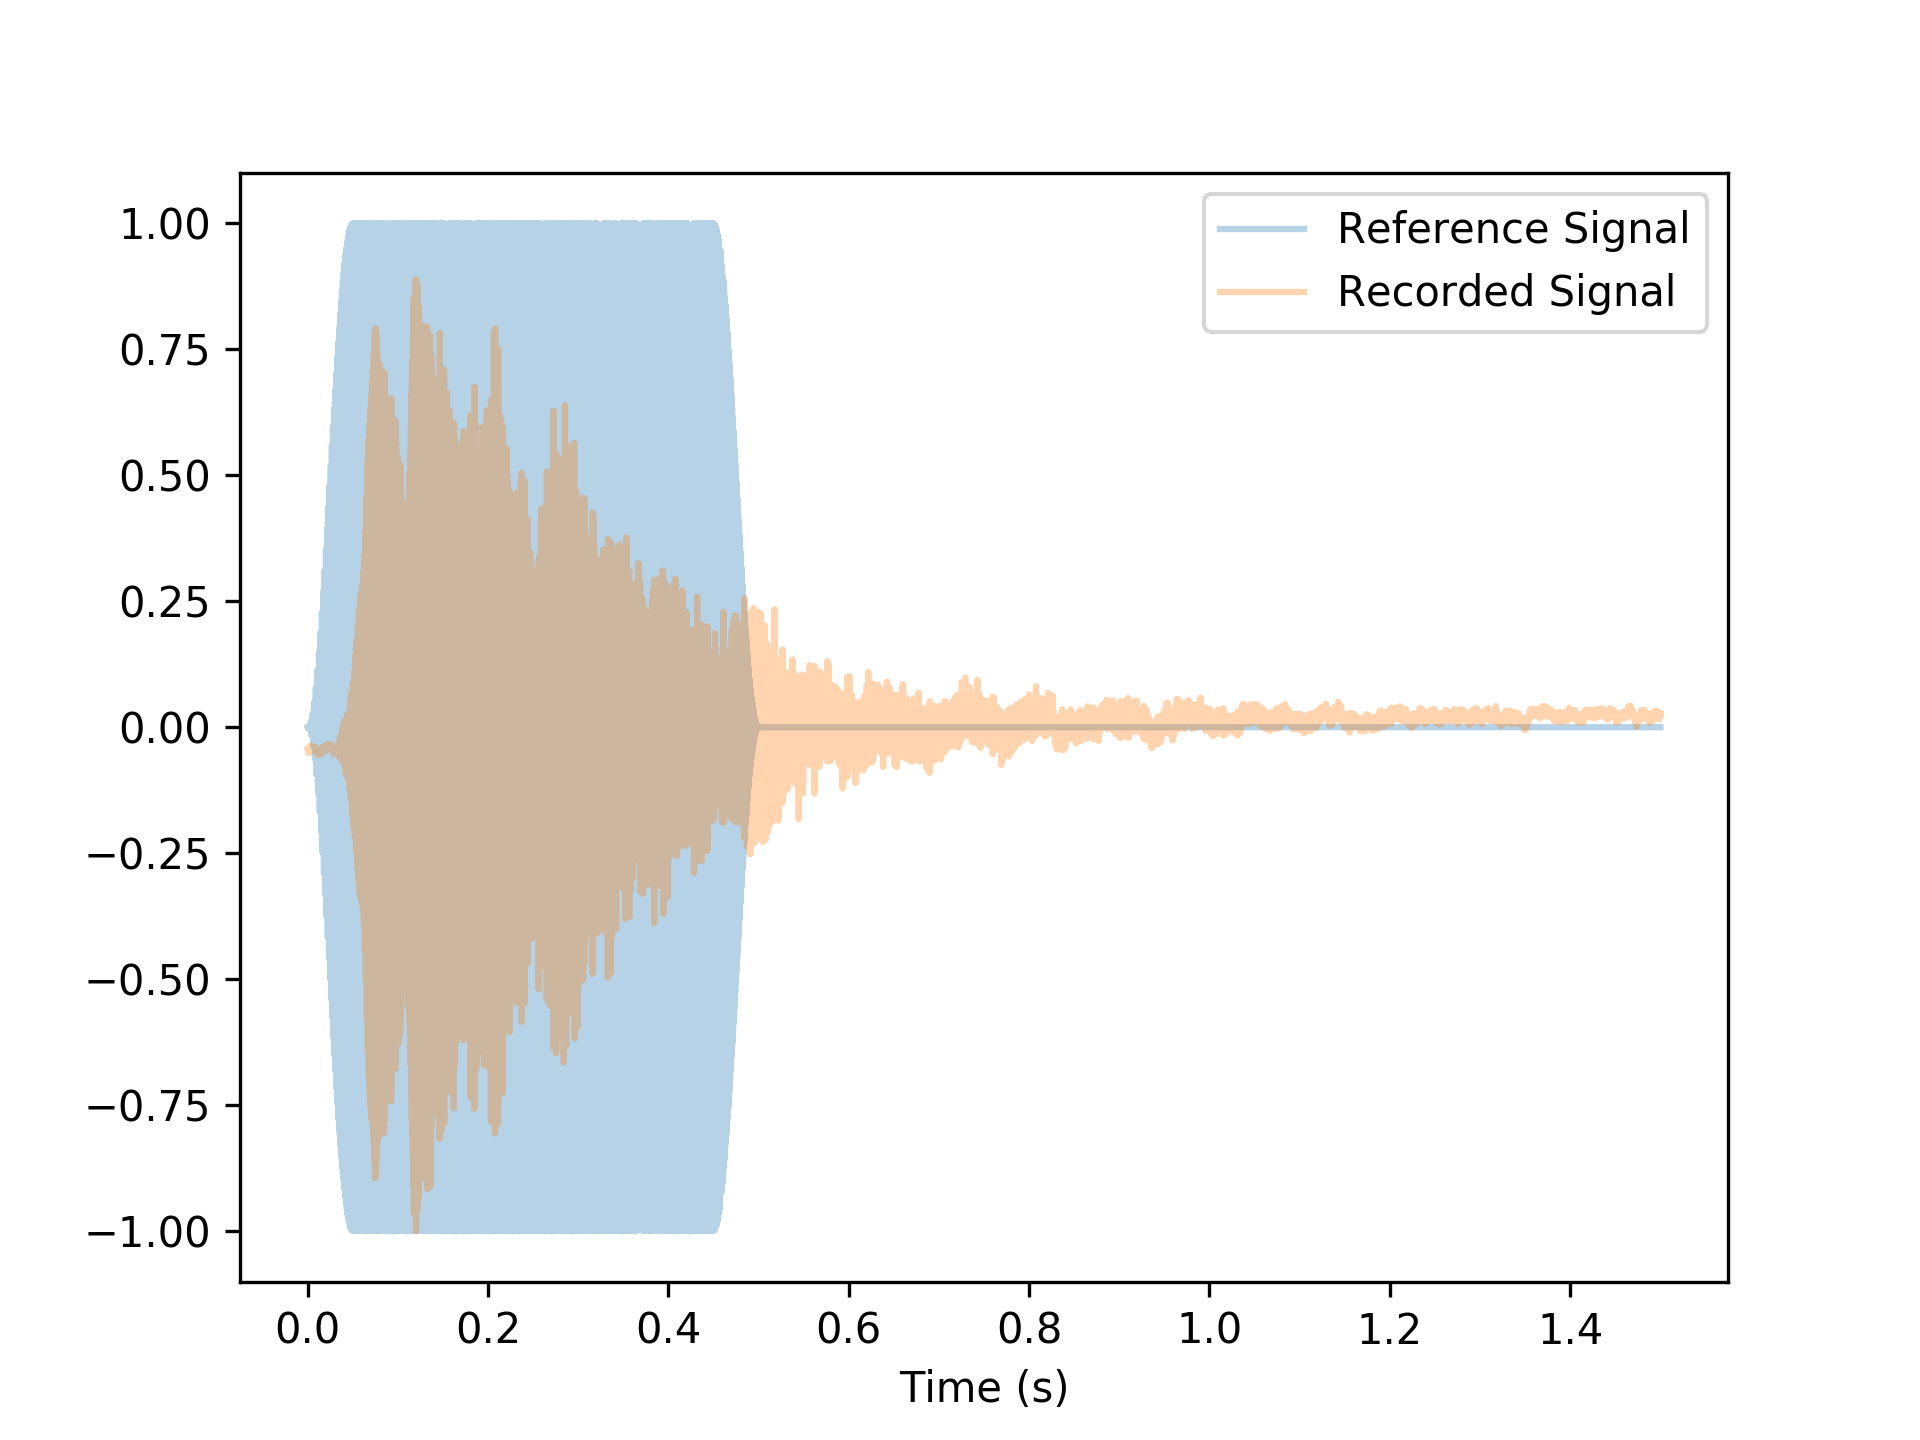
\includegraphics[width=0.45\textwidth]{images/signal_example.png} }}
	\subfloat{{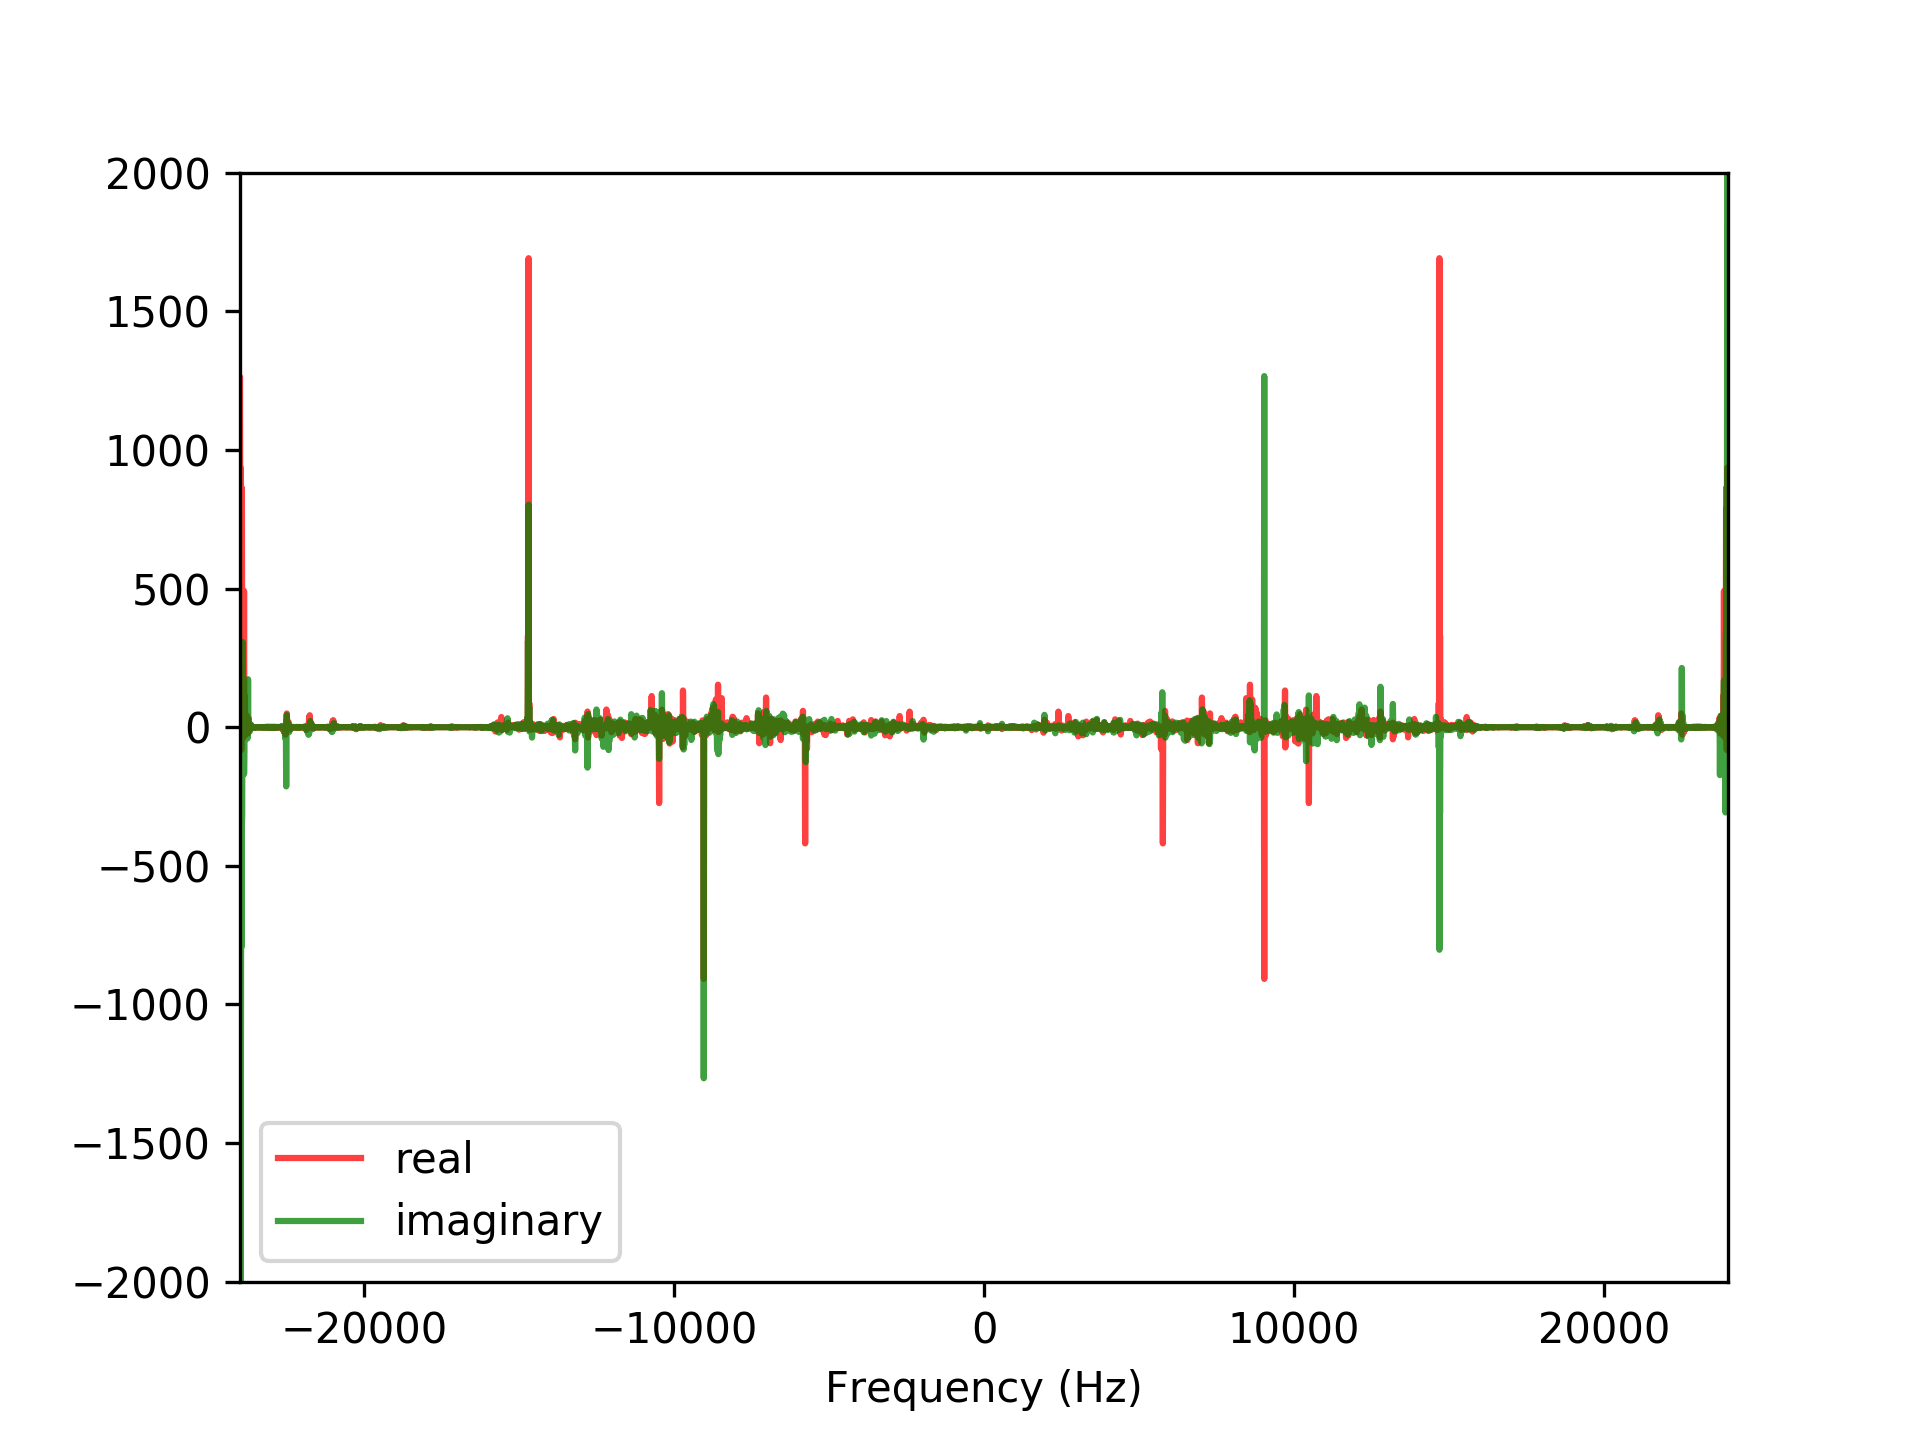
\includegraphics[width=0.45\textwidth]{images/response_example.png} }}
	\caption{
		On the left in blue, the chirp signal with a frequency starting at 200 Hz and going up to 4000 Hz linearly. The chirp signal is 0.5 seconds long and was multiplied with a Tukey window. That implies a smooth chirp signal which starts and ends with zero. That prevents clicking sounds. In orange the recorded signal and on the right the RIR. Because of the sampling rate of 48000 Hz, the impulse response shows frequencies up to 24000 Hz. 
	}
	\label{fig:signal_response_example}
\end{figure}

But it seems that the phase isn't necessary for this use case. When looking at the peaks of the magnitude, RIR at the same position will look similar as illustrated in Figure \ref{fig:response-same-room-same-pos} which is expectable when looking at the work of Dokmanic \cite{dokmanic_roomrecslam_2016}. Also expectable is that the peaks in magnitude are at a different position when changing the room which can be seen in Figure \ref{fig:response-different-room}. More interesting is the RIR of the same room but different positions. It turns out that the RIR is recognizably different in the same room but in different positions which can be seen in Figure \ref{fig:response-same-room-different-pos}. Also interesting, peaks in the same room but different positions seem to be at similar positions when moving around (like in Figure \ref{fig:dokmanic_roomrecslam}). But when changing the room the peak characteristic will change. That probably leads to a continuous function which is usable for SLAM purposes.

\begin{figure}[h!]
	\centering
	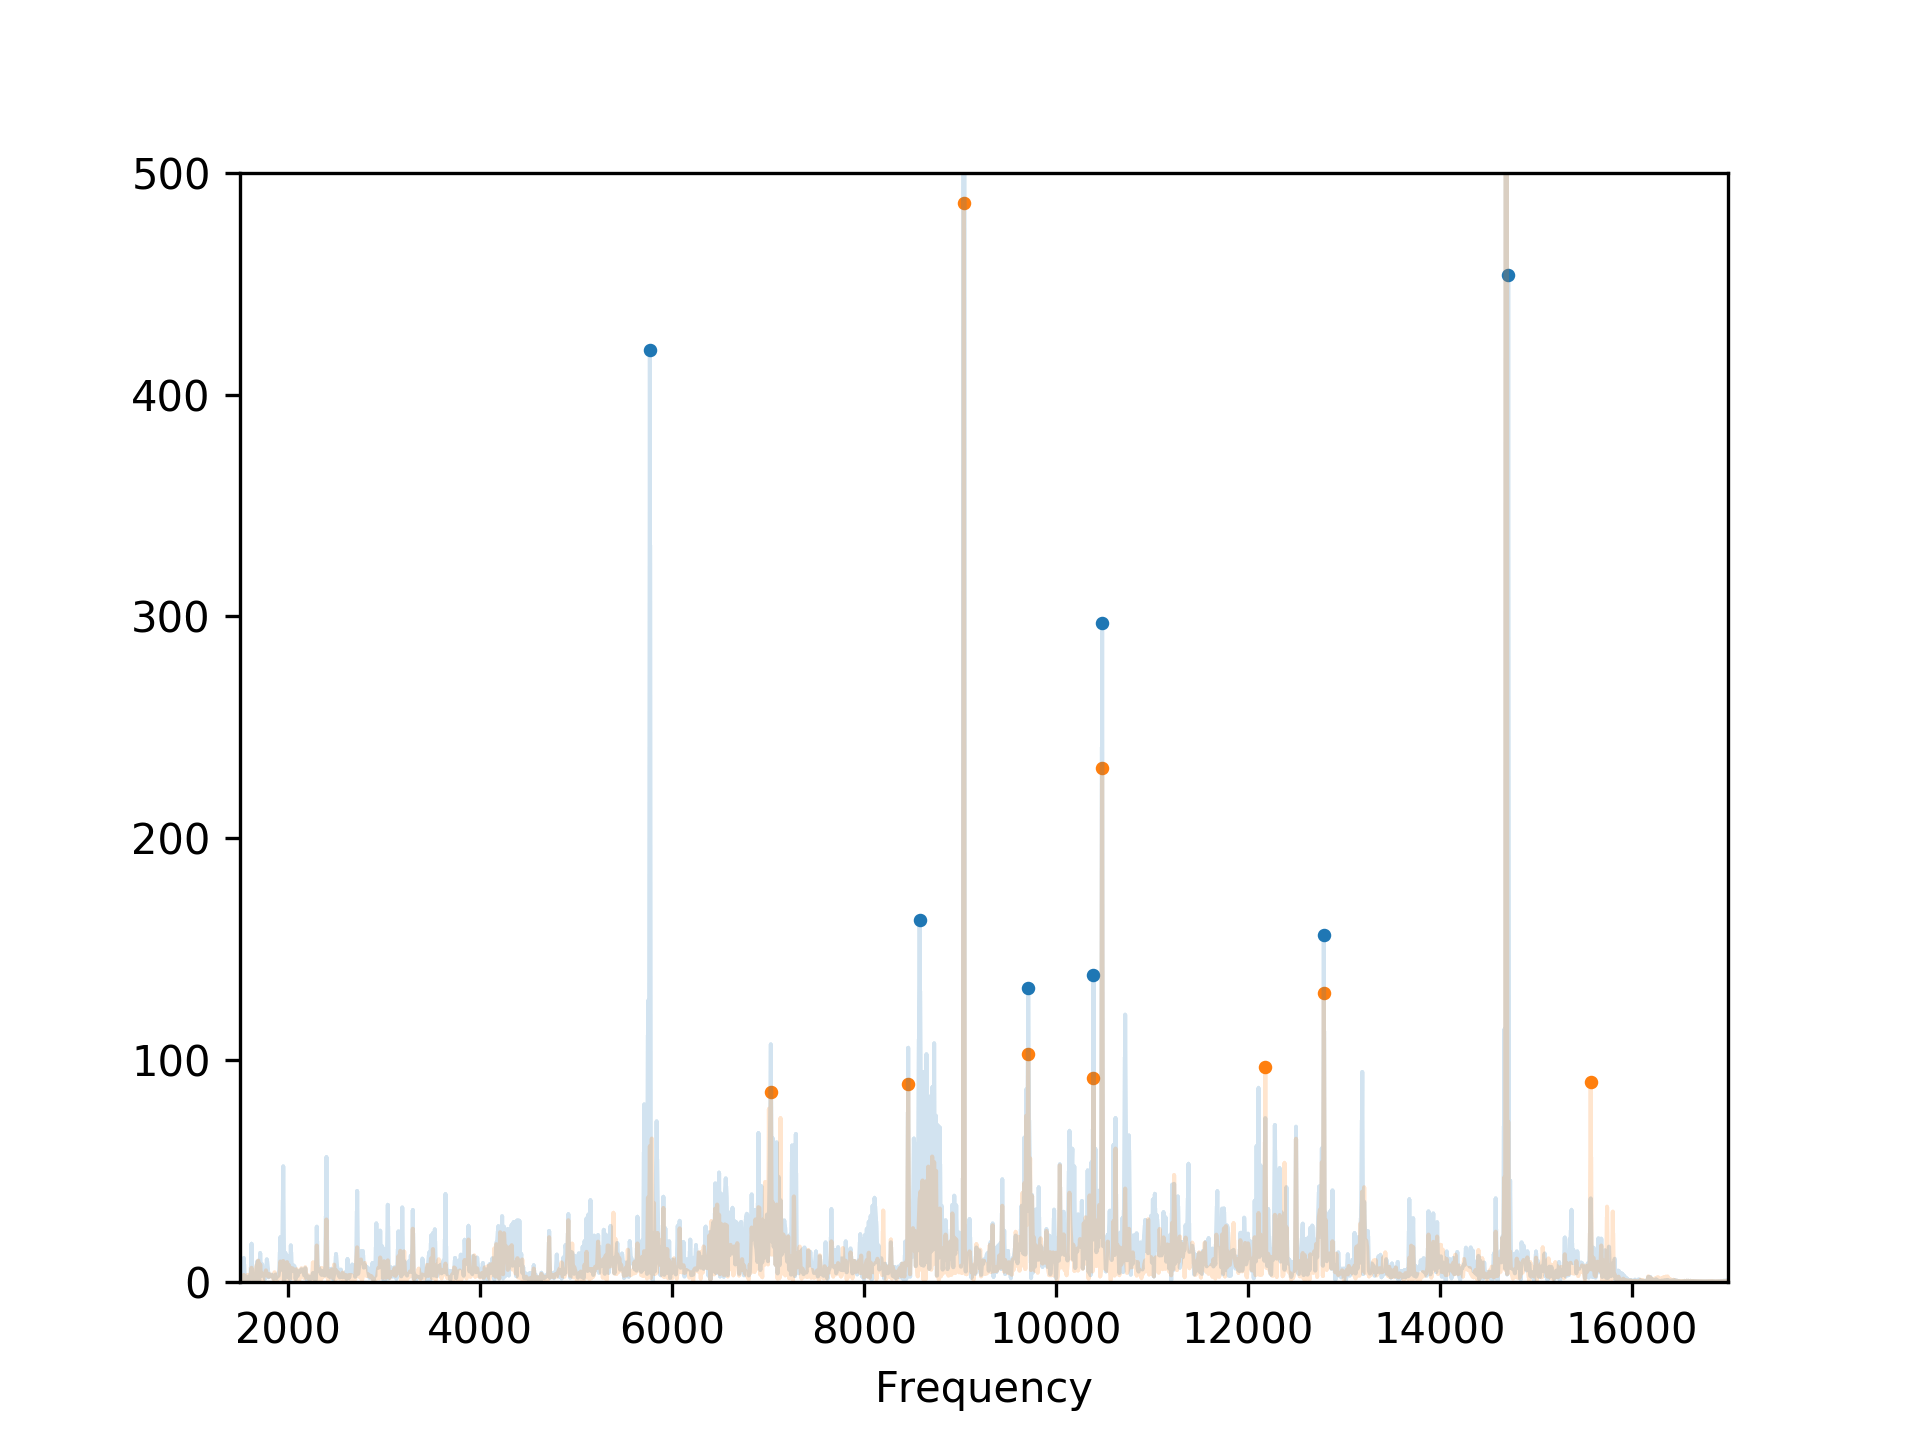
\includegraphics[width=0.92\textwidth]{images/response-same-room-same-pos.png}
	\caption{
		Two RIR of the position but different times. Notice, most of the peaks are at the same position.
	}
	\label{fig:response-same-room-same-pos}
\end{figure}

\begin{figure}[h!]
	\centering
	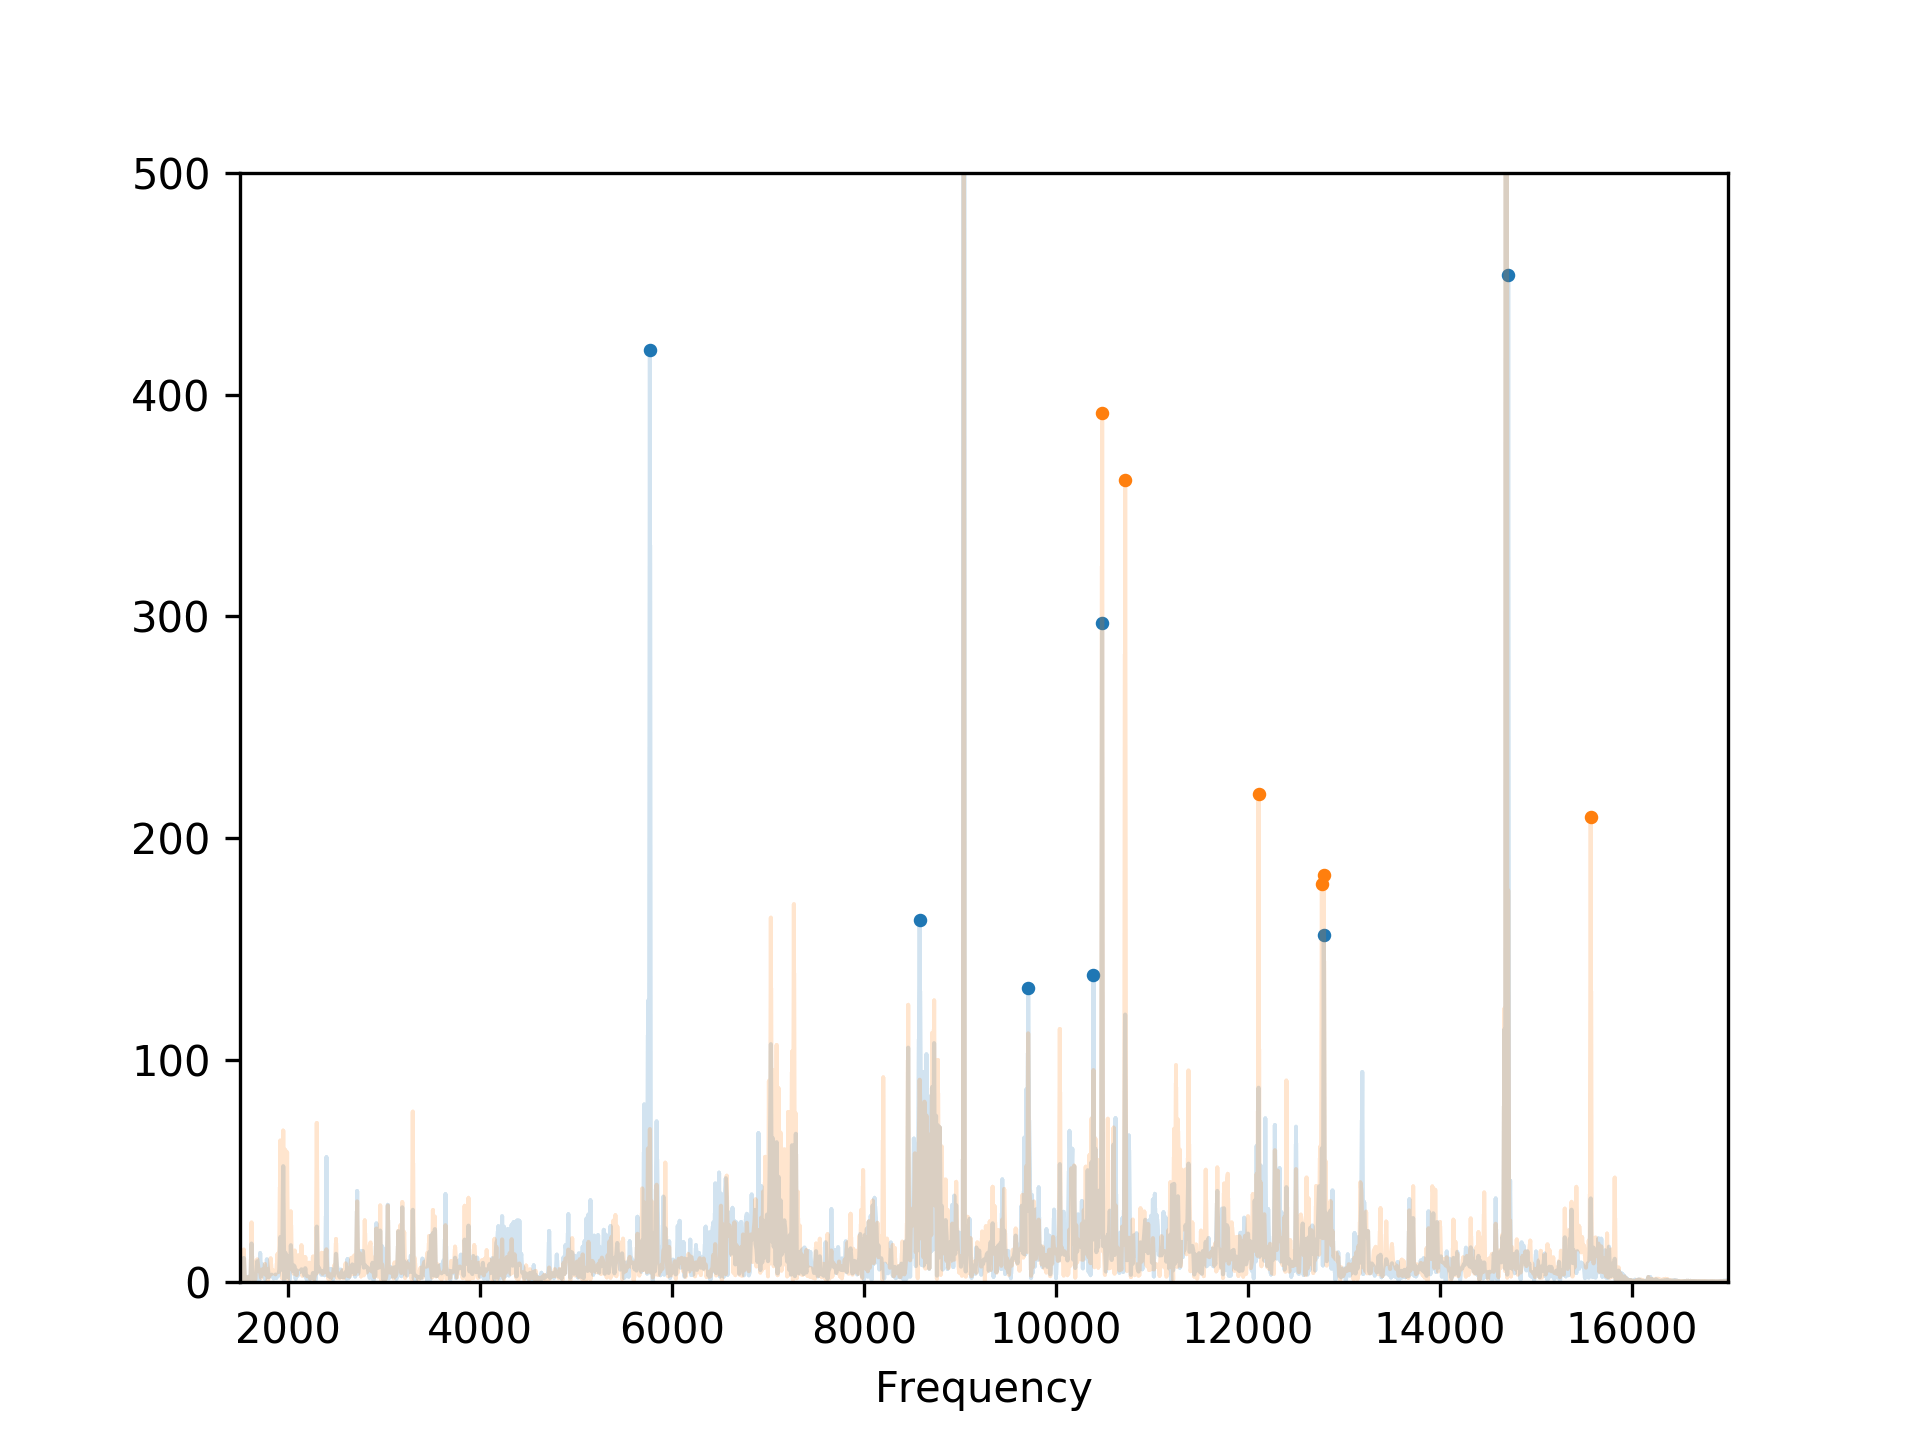
\includegraphics[width=0.92\textwidth]{images/response-different-room.png}
	\caption{
		RIR of two different rooms. Notice, the peak characteristic has changed.
	}
	\label{fig:response-different-room}
\end{figure}

\begin{figure}[h!]
	\centering
	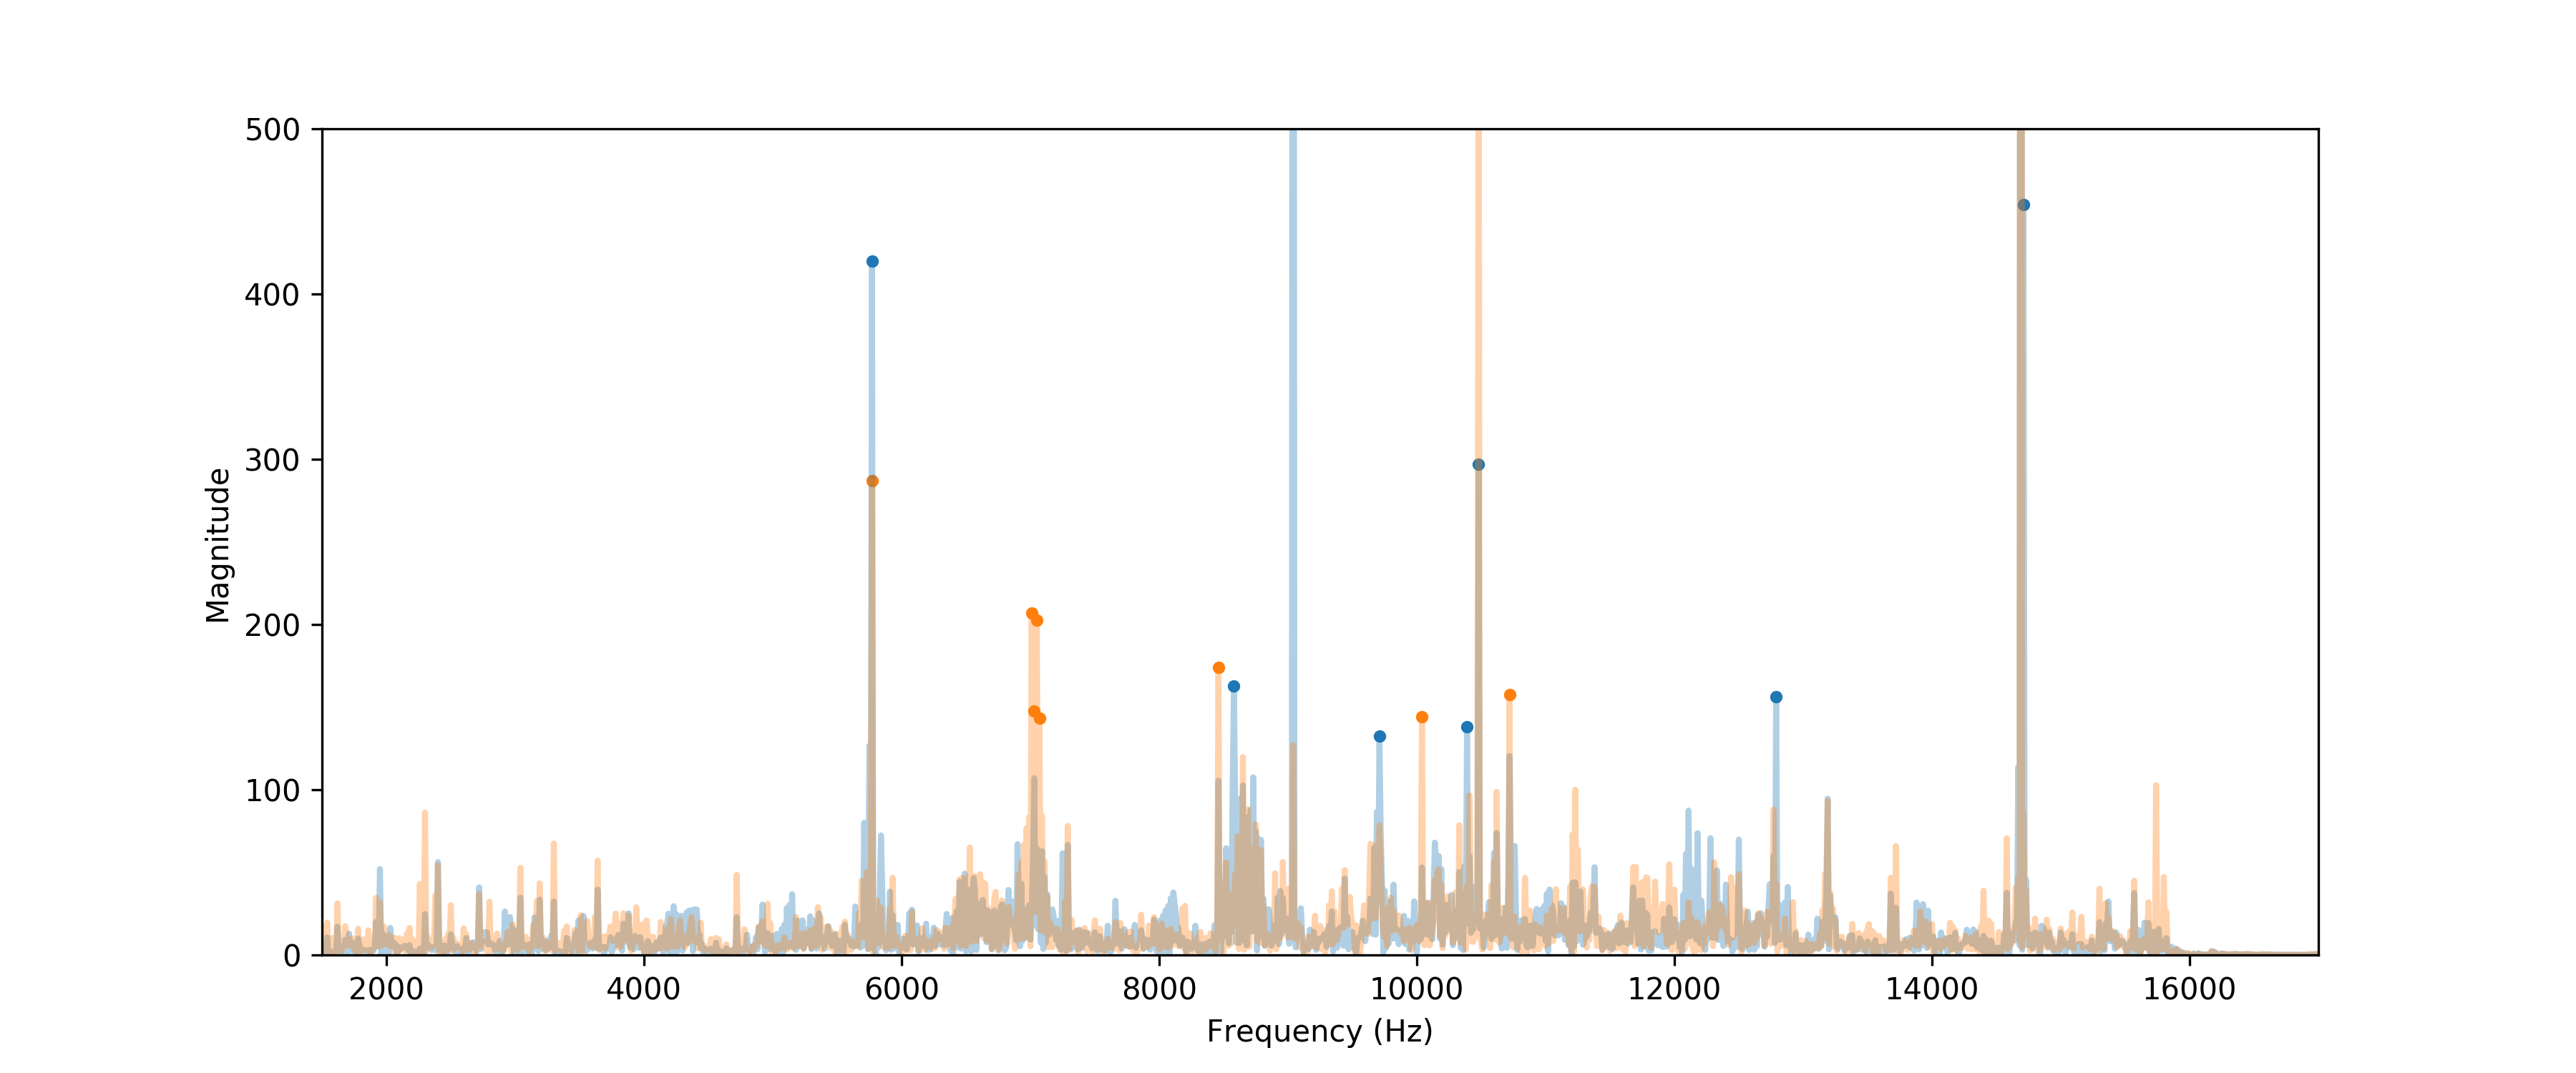
\includegraphics[width=0.92\textwidth]{images/response-same-room-different-pos.png}
	\caption{
		Two RIR of the same room but different positions. Notice, the change in peaks is recognizable but some peaks are only shifted slightly.
	}
	\label{fig:response-same-room-different-pos}
\end{figure}
